\documentclass[11pt,a4paper]{article}

% Packages
\usepackage[utf8]{inputenc}
\usepackage[T1]{fontenc}
\usepackage{amsmath,amssymb,amsthm}
\usepackage{mathtools}
\usepackage{physics}
\usepackage{graphicx}
\usepackage{hyperref}
\usepackage{cleveref}
\usepackage{booktabs}
\usepackage{caption}
\usepackage{subcaption}
\usepackage[margin=1in]{geometry}
\usepackage{algorithm}
\usepackage{algpseudocode}
\usepackage{tikz}
\usetikzlibrary{matrix,positioning,arrows.meta}

% Theorem environments
\newtheorem{definition}{Definition}
\newtheorem{theorem}{Theorem}
\newtheorem{proposition}{Proposition}
\newtheorem{lemma}{Lemma}
\newtheorem{corollary}{Corollary}
\newtheorem{remark}{Remark}
\newtheorem{example}{Example}

% NA0 notation
\newcommand{\NA}{\mathrm{NA0}}
\newcommand{\debt}{\mathcal{D}}
\newcommand{\remainder}{\mathcal{R}}
\newcommand{\policy}{\Pi}
\newcommand{\proj}{\mathcal{P}}

% Title
\title{Non-Atomic Zero: A Unified Theory of Projection-Honest Computation}

\author{
  David Ingle\thanks{Preprint draft. Comments welcome at \texttt{Dave@vertrule.com}.}\\
  VertRule Inc.
}

\date{\today}

\begin{document}

\maketitle

\begin{abstract}
We introduce \emph{Non-Atomic Zero} ($\NA$), a mathematical framework that makes
explicit the information discarded by projection and totalization operations.
Standard computational practice treats projection as atomic---collapsing
high-dimensional objects to scalars while silently discarding context. $\NA$
instead represents such operations as structured objects $\NA\langle \debt,
\remainder; \policy \rangle$ carrying: (1) the discarded information (\emph{debt}
$\debt$), (2) the retained value (\emph{remainder} $\remainder$), and (3) the
projection rule (\emph{policy} $\policy$). We demonstrate the framework across
multiple domains: divergent series regularization (where $\NA$ clarifies the sense
in which $1+2+3+\cdots = -1/12$), signal processing (where baseline subtraction
policies induce correlated debt-remainder variations), spectral analysis
(where exporting projectors avoids eigenvector instabilities), and reduced
quantum dynamics (where memory effects arise as correction terms for naive
projection). Our experiments show that policy changes produce predictable,
measurable shifts in both debt and remainder, enabling detection of
projection-induced artifacts. We propose $\NA$ as a foundation for
\emph{projection-honest} computation, where all totalization debt is explicitly
tracked and auditable.
\end{abstract}

\section{Introduction}
\label{sec:introduction}

Projection is ubiquitous in scientific computation. Whenever we reduce a
high-dimensional object to a summary statistic, fit a model to data, trace out
environmental degrees of freedom, or regularize a divergent series, we perform a
projection---discarding some information to obtain a tractable result. Standard
practice treats such operations as atomic: the projection produces a scalar or
low-dimensional object, and the discarded information vanishes.

This paper argues that treating projection as atomic is computationally
hazardous. The discarded information does not vanish; it becomes implicit debt
that can resurface as apparent disagreements between methods, spurious
``tensions'' between experiments, or artifacts mistaken for physical effects.

We introduce \emph{Non-Atomic Zero} ($\NA$), a framework that makes projection
debt explicit. An $\NA$ object has the form:
\begin{equation}
  \NA\langle \debt, \remainder; \policy \rangle
\end{equation}
where $\debt$ is the discarded information (debt), $\remainder$ is the retained
value (remainder), and $\policy$ is the projection rule (policy). The zero in
``Non-Atomic Zero'' reflects the fact that these objects generalize the notion of
``collapsing to zero''---the standard treatment makes the debt contribution zero
by fiat, while $\NA$ preserves it.

\subsection{Projection as a Source of Artifacts}

Three examples motivate the framework:

\paragraph{Divergent Series.} The statement $1 + 2 + 3 + \cdots = -1/12$ is
notorious for provoking confusion. The series diverges; how can it equal a
negative fraction? The answer is that this is not a statement about convergence
but about \emph{regularization}---a specific projection policy (zeta-function
regularization or Ramanujan summation) that extracts a finite part from a
divergent object. Different regularization schemes can yield different values.
The $\NA$ framework makes explicit what is discarded: the divergent part becomes
debt, the finite part becomes remainder, and the regularization scheme is the
policy.

\paragraph{Background Subtraction.} In astronomy and spectroscopy, estimating a
signal often requires subtracting a model of the background. Different baseline
models (linear, polynomial, spline) fitted to the same ``source-free'' regions
can yield significantly different signal estimates. The
disagreement is not statistical noise but projection policy disagreement: each
model class extrapolates differently from the fitting regions to the signal
regions. $\NA$ represents this as debt (the model's extrapolation uncertainty)
correlated with remainder (the estimated signal).

\paragraph{Quantum Reduced Dynamics.} The Nakajima-Zwanzig
equation~\cite{nakajima1958,zwanzig1960} provides the exact reduced dynamics of
a quantum system coupled to an environment:
\begin{equation}
  \frac{d\rho_S}{dt} = \mathcal{L}_S \rho_S + \int_0^t K(t-\tau) \rho_S(\tau)\, d\tau + I(t)
\end{equation}
The memory kernel $K(t)$ and inhomogeneity $I(t)$ are precisely the correction
terms required because the naive projected dynamics (first term alone) discards
system-environment correlations. In $\NA$ terms, tracing out the environment
creates debt; the memory kernel is the back-action of that debt on the reduced
system.

\subsection{Contributions}

This paper makes five contributions:

\begin{enumerate}
  \item \textbf{Formalization}: We define the $\NA$ algebra, including
    composition rules and the ``projection timing sensitivity'' (PTS) diagnostic
    that detects non-commutative projection effects.

  \item \textbf{Divergence Application}: We show how $\NA$ clarifies famous
    regularized sums, making the debt-remainder decomposition explicit.

  \item \textbf{Signal Processing Experiments}: We demonstrate experimentally
    that policy variations induce correlated debt-remainder changes, and that
    these correlations are detectable.

  \item \textbf{Spectral Analysis}: We introduce projection-honest spectral
    methods that export projectors rather than eigenvectors, avoiding sign-flip
    and degeneracy artifacts.

  \item \textbf{Quantum Dynamics}: We show that, in the Jaynes-Cummings setting
    studied here, the $\NA$ correction term aligns with the Nakajima--Zwanzig
    memory contribution and can be expressed in the same structural form.
\end{enumerate}

\subsection{Paper Organization}

\Cref{sec:na0-algebra} formalizes the $\NA$ framework.
\Cref{sec:divergence} applies it to divergent series.
\Cref{sec:signal} presents the signal processing experiments.
\Cref{sec:spectral} develops projection-honest spectral methods.
\Cref{sec:quantum} demonstrates the quantum dynamics application.
\Cref{sec:discussion} discusses implications and future work.

\subsection{Related Work}

The $\NA$ framework connects to several established research areas:

\paragraph{Divergent Series and Regularization.}
Hardy's foundational treatment of divergent series~\cite{hardy1949} and Ramanujan's summation methods~\cite{ramanujan1927} establish the classical theory. The Hadamard finite part~\cite{hadamard1923} and distributional approaches~\cite{gelfand1964} provide rigorous frameworks for extracting finite values. The Casimir effect~\cite{casimir1948} demonstrates physical relevance. $\NA$ provides a common notation for these techniques, making the policy-dependence of ``values'' explicit.

\paragraph{Baseline Subtraction and Model Selection.}
Baseline estimation in spectroscopy~\cite{lieber2003,eilers2010} and signal processing~\cite{titterington1985} involves model-class choices that are often treated as preprocessing. The $\NA$ framework treats these as projection policies whose effects propagate into downstream results.

\paragraph{Spectral Analysis and Subspace Stability.}
The Davis-Kahan theorem~\cite{daviskahan1970} bounds eigenvector perturbation but does not resolve sign/basis ambiguity. Subspace angles and distances~\cite{ye2016,stewart1990} provide basis-independent metrics. PCA and spectral clustering~\cite{jolliffe2016,golub1973} inherit these ambiguities. $\NA$-aware methods export projectors rather than eigenvectors, avoiding artifacts.

\paragraph{Open Quantum Systems.}
The Nakajima-Zwanzig projection operator technique~\cite{nakajima1958,zwanzig1960} and related methods (Lindblad~\cite{lindblad1976,gorini1976}, time-convolutionless~\cite{shibata1977}) provide exact or approximate reduced dynamics. Recent work~\cite{breuer2009,chruściński2022,breuer2002} characterizes non-Markovianity. The Jaynes-Cummings model~\cite{jaynes1963} serves as a standard test case. $\NA$ generalizes the insight that projection creates correctable debt beyond the quantum setting.

\section{The NA0 Algebra}
\label{sec:na0-algebra}

We formalize the $\NA$ framework as an algebraic structure that tracks
projection debt alongside retained values.

\begin{table}[t]
\centering
\caption{Summary of NA0 notation.}
\label{tab:notation}
\begin{tabular}{@{}ll@{}}
\toprule
\textbf{Symbol} & \textbf{Meaning} \\
\midrule
$\mathcal{X}$ & Ambient space of objects under projection \\
$\mathcal{R}_\Pi$ & Remainder space for policy $\Pi$ \\
$\Pi$ & Policy (projection rule / totalization scheme) \\
$r_\Pi : \mathcal{X} \to \mathcal{R}_\Pi$ & Remainder extractor \\
$\ell_\Pi : \mathcal{R}_\Pi \to \mathcal{X}$ & Lift (reconstruction map) \\
$q_\Pi(X) = X - \ell_\Pi(r_\Pi(X))$ & Induced debt map \\
$D$ & Debt component (lives in $\mathcal{X}$) \\
$R$ & Remainder component (lives in $\mathcal{R}_\Pi$) \\
$\NA\langle D, R; \Pi\rangle$ & NA0 object: debt, remainder, policy \\
$P_\Pi(X)$ & NA0 projection operator \\
$\mathrm{Rec}_\Pi$ & Reconstruction: $D + \ell_\Pi(R)$ \\
$\mathrm{Total}$ & Totalization: extract $R$, discard $D$ \\
$\mathrm{PTS}_R$ & Projection timing sensitivity (remainder channel) \\
$\mathrm{DTR}$ & Debt-to-Remainder Ratio (admissibility criterion) \\
$\mathrm{PTSBudget}$ & Relative PTS error (admissibility criterion) \\
$\tau_{\mathrm{DTR}}, \tau_{\mathrm{PTS}}$ & Admissibility thresholds (default: 0.1, 0.05) \\
\bottomrule
\end{tabular}
\end{table}

\subsection{Basic Definitions}

We begin with a minimal model that makes ``debt'' and ``remainder'' well-typed.
This model is sufficient for the additive projection cases used throughout the paper;
other domains can be treated as extensions by replacing $+$ with an explicit reconstruction operator.

\begin{definition}[Policy, remainder extractor, and lift]
  \label{def:policy_rl}
  Fix an ambient space $\mathcal{X}$ (a vector space or abelian group) for objects $X$ under consideration.
  A policy $\Pi$ specifies:
  (i) a remainder space $\mathcal{R}_\Pi$ (also a vector space or abelian group),
  (ii) a remainder extractor $r_\Pi:\mathcal{X}\to\mathcal{R}_\Pi$,
  and (iii) a lift (reconstruction map) $\ell_\Pi:\mathcal{R}_\Pi\to\mathcal{X}$.
  We require $\ell_\Pi$ to be a right-inverse on the image of $r_\Pi$:
  \[
    r_\Pi(\ell_\Pi(R)) = R \quad \forall R \in \mathrm{Im}(r_\Pi).
  \]
  In the minimal additive model used throughout this paper, we further require $r_\Pi$ and $\ell_\Pi$
  to be linear (or additive homomorphisms). This ensures that the PTS identity
  (\Cref{prop:pts-debt}) and related results hold.
\end{definition}

\begin{definition}[Debt map and NA0 object]
  \label{def:na0_minimal}
  Given $(r_\Pi,\ell_\Pi)$, define the lifted remainder in $\mathcal{X}$ as
  \[
    \tilde R_\Pi(X) \coloneqq \ell_\Pi(r_\Pi(X)).
  \]
  Define the induced debt map
  \[
    q_\Pi(X) \coloneqq X - \tilde R_\Pi(X),
  \]
  where subtraction is taken in $\mathcal{X}$ (thus this minimal model assumes $\mathcal{X}$ supports an additive structure).
  An \emph{NA0 object} is
  \[
    \NA\langle D, R; \Pi \rangle,
  \]
  where $R=r_\Pi(X)\in\mathcal{R}_\Pi$ and $D=q_\Pi(X)\in\mathcal{X}$ for some $X\in\mathcal{X}$.
\end{definition}

\begin{definition}[Reconstruction and well-posedness]
  \label{def:reconstruct}
  Reconstruction under policy $\Pi$ is the map
  \[
    \mathrm{Rec}_\Pi(\NA\langle D,R;\Pi\rangle) \coloneqq D + \ell_\Pi(R).
  \]
  In the minimal additive model,
  \[
    \mathrm{Rec}_\Pi(\NA\langle q_\Pi(X), r_\Pi(X);\Pi\rangle)=X
  \]
  holds identically. We call $\Pi$ \emph{well-posed} for NA0 bookkeeping if $\ell_\Pi$ is specified and $q_\Pi(X)$ is defined for all $X$ of interest.
\end{definition}

\begin{definition}[Canonical debt representations]
  \label{def:canonical_debt}
  In practice, the debt component $D$ is not arbitrary. Common well-posed representations include:
  \begin{itemize}
    \item \textbf{Complement residual debt (additive):} $D=q_\Pi(X)\in\mathcal{X}$ induced by an explicit lift $\ell_\Pi$.
    \item \textbf{Uncertainty debt:} $D$ as a distribution/covariance/interval object plus the assumptions required to interpret it (model class, regularization, priors).
    \item \textbf{Sufficient-statistics debt:} $D$ as the minimal metadata and statistics required to recompute or re-totalize under alternate policies (e.g., fit diagnostics, hyperparameters, and restricted residuals).
  \end{itemize}
  All debt representations used in this paper are required to be deterministically serializable and comparable under a declared metric.
\end{definition}

\begin{remark}[Well-posedness criteria for debt]
  \label{rem:wellposed}
  To distinguish NA0 from informal ``residual logging,'' debt must satisfy:
  \begin{enumerate}
    \item \textbf{Typed}: $D$ lives in a declared space with defined operations.
    \item \textbf{Comparable}: A metric or norm is specified for measuring debt magnitude.
    \item \textbf{Serializable}: $D$ admits a canonical, deterministic encoding.
    \item \textbf{Policy-addressable}: $D$ includes sufficient metadata to re-totalize under alternate policies or to trigger fail-closed behavior.
  \end{enumerate}
  These criteria ensure that debt is a first-class computational object, not merely a comment or annotation.
\end{remark}

\begin{definition}[Totalization]
  \label{def:totalization}
  \emph{Totalization} is the operation that extracts only the remainder,
  discarding the debt:
  \begin{equation}
    \mathrm{Total}(\NA\langle D, R; \Pi \rangle) = R
  \end{equation}
  Totalization converts an $\NA$ object back to a scalar (or low-dimensional
  object), losing the debt information.
\end{definition}

Standard computational practice implicitly totalizes at every projection step.
$\NA$ defers totalization, preserving debt for downstream analysis.

\subsection{Composition in the minimal additive model}

Composition is induced by the policy maps $(r_\Pi,\ell_\Pi)$ and may fail to exist if types do not align.

\begin{definition}[Sequential policy application]
  \label{def:policy_apply}
  For a policy $\Pi$ with maps $(r_\Pi,\ell_\Pi)$, define the NA0 projection operator
  \[
    P_\Pi(X)\coloneqq \NA\langle q_\Pi(X), r_\Pi(X); \Pi\rangle.
  \]
  Given two policies $\Pi_1,\Pi_2$ defined over a shared ambient space $\mathcal{X}$,
  the sequential policy $\Pi_{2\circ 1}$ is defined whenever $r_{\Pi_2}$ is valid on $\mathcal{X}$.
  In that case, we define
  \[
    P_{\Pi_{2\circ 1}}(X)\coloneqq \NA\langle q_{\Pi_2}(X), r_{\Pi_2}(X); \Pi_2\rangle,
  \]
  and note that NA0 bookkeeping is threaded by explicitly retaining the earlier debt objects rather than discarding them.
\end{definition}

\begin{remark}
  This definition replaces informal ``$\oplus$''/``$\otimes$'' composition. In the additive model, composition is not arbitrary:
  it is determined by declared extract/lift pairs and their shared ambient space. Later sections treat non-additive cases as extensions by declaring a reconstruction operator in place of $+$.
\end{remark}

\begin{example}[Worked composition: baseline then threshold]
  \label{ex:composition}
  Consider a signal $X \in \mathbb{R}^n$ processed by two sequential projections:
  \begin{enumerate}
    \item \textbf{Baseline subtraction} $\Pi_1$: Fit a polynomial $p(x)$ to edge regions, subtract it.
      \begin{itemize}
        \item $r_{\Pi_1}(X) = X - p$ (baseline-subtracted signal)
        \item $\ell_{\Pi_1}(R) = R$ (identity lift into $\mathbb{R}^n$)
        \item $q_{\Pi_1}(X) = p$ (the fitted baseline is debt)
      \end{itemize}
    \item \textbf{Thresholding} $\Pi_2$: Zero values below threshold $\tau$.
      \begin{itemize}
        \item $r_{\Pi_2}(Y) = Y \cdot \mathbf{1}_{Y > \tau}$ (thresholded signal)
        \item $\ell_{\Pi_2}(R) = R$ (identity lift)
        \item $q_{\Pi_2}(Y) = Y \cdot \mathbf{1}_{Y \leq \tau}$ (sub-threshold values are debt)
      \end{itemize}
  \end{enumerate}

  Applying $\Pi_1$ then $\Pi_2$ to $X$:
  \[
    P_{\Pi_2}(P_{\Pi_1}(X)) = \NA\Big\langle q_{\Pi_2}(X-p),\; r_{\Pi_2}(X-p);\; \Pi_2 \Big\rangle
  \]
  with accumulated debt $(p, q_{\Pi_2}(X-p))$---the baseline \emph{and} the sub-threshold residuals.

  NA0 bookkeeping threads both debt components. Standard practice discards $p$ after step 1, losing the ability to diagnose whether apparent ``signal'' came from baseline model choice or thresholding.

  \textbf{Fail-closed condition}: If $\|p\| > \theta_1$ (baseline too large) or $\|q_{\Pi_2}\| > \theta_2$ (too much thresholded), refuse to totalize.
\end{example}

\begin{figure}[t]
\centering
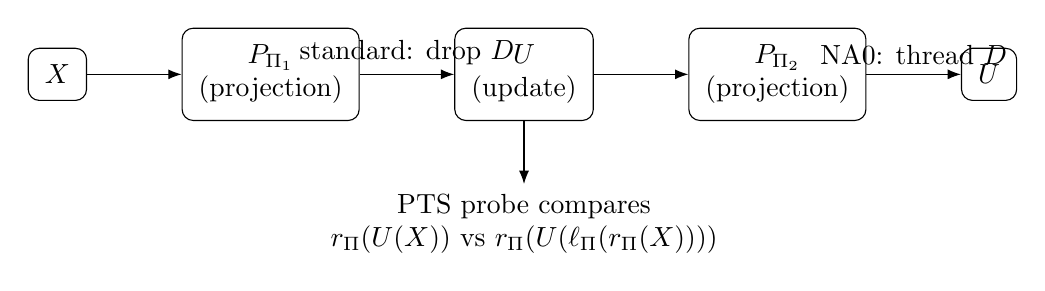
\begin{tikzpicture}[
  node distance=12mm,
  box/.style={draw, rounded corners, inner sep=6pt, align=center},
  arr/.style={-Latex}
]
\node[box] (x0) {$X$};
\node[box, right=of x0] (p1) {$P_{\Pi_1}$\\(projection)};
\node[box, right=of p1] (u1) {$U$\\(update)};
\node[box, right=of u1] (p2) {$P_{\Pi_2}$\\(projection)};
\node[box, right=of p2] (u2) {$U$};
\draw[arr] (x0) -- (p1);
\draw[arr] (p1) -- node[above]{standard: drop $D$} (u1);
\draw[arr] (u1) -- (p2);
\draw[arr] (p2) -- node[above]{NA0: thread $D$} (u2);
\node[below=8mm of u1, align=center] (pts) {PTS probe compares\\$r_\Pi(U(X))$ vs $r_\Pi(U(\ell_\Pi(r_\Pi(X))))$};
\draw[arr] (u1) -- (pts);
\end{tikzpicture}
\caption{Projection-honest computation threads debt objects across repeated projections. PTS provides an operational diagnostic for projection timing sensitivity.}
\label{fig:pipeline}
\end{figure}

\subsection{Projection Timing Sensitivity}

A key diagnostic for projection effects is non-commutativity with other
operations.

\begin{definition}[Projection Timing Sensitivity (typed remainder form)]
  \label{def:pts_typed}
  Let $\Pi$ be a policy with $(r_\Pi,\ell_\Pi)$ and let $U:\mathcal{X}\to\mathcal{X}$ be an update/evolution operator.
  Define the remainder-channel PTS:
  \[
    \mathrm{PTS}_R(\Pi,U,X) \coloneqq r_\Pi(U(X)) - r_\Pi\!\big(U(\ell_\Pi(r_\Pi(X)))\big),
  \]
  which compares evolve-then-extract vs extract-then-lift-then-evolve-then-extract.
  We say PTS is present when $\mathrm{PTS}_R(\Pi,U,X)\neq 0$ under a declared metric on $\mathcal{R}_\Pi$.
\end{definition}

\begin{proposition}[Debt form of PTS under additive reconstruction]
  \label{prop:pts-debt}
  Assume the policy $\Pi$ admits additive reconstruction in $\mathcal{X}$
  (so $X = q_\Pi(X) + \ell_\Pi(r_\Pi(X))$), and assume $U$ is linear over $+$.
  Then the remainder PTS satisfies:
  \begin{equation}
    \mathrm{PTS}_R(\Pi, U, X) = r_\Pi(U(q_\Pi(X))),
  \end{equation}
  i.e., PTS measures how the evolved debt projects back onto the remainder channel.
\end{proposition}

\begin{proof}
  Write $R = r_\Pi(X)$ and $D = q_\Pi(X) = X - \ell_\Pi(R)$.
  Then $U(X) = U(D) + U(\ell_\Pi(R))$ by linearity.
  We have:
  \begin{align}
    \mathrm{PTS}_R(\Pi,U,X)
      &= r_\Pi(U(X)) - r_\Pi(U(\ell_\Pi(R))) \\
      &= r_\Pi(U(D) + U(\ell_\Pi(R))) - r_\Pi(U(\ell_\Pi(R))) \\
      &= r_\Pi(U(D)),
  \end{align}
  where the last step uses linearity of $r_\Pi$ (which follows from the additive model).
\end{proof}

This shows that PTS measures how debt transforms under evolution and projects back.

\subsection{Projection Non-Transparency}

The following theorem establishes that non-zero PTS implies provable information loss
from naive projection---loss that cannot be recovered without access to the debt.

\begin{theorem}[Projection Non-Transparency]
  \label{thm:non-transparency}
  Let $\Pi$ be a well-posed policy with $(r_\Pi, \ell_\Pi, q_\Pi)$ satisfying
  additive reconstruction in a normed space $(\mathcal{X}, \|\cdot\|)$.
  Let $U: \mathcal{X} \to \mathcal{X}$ be linear, and let $\|\cdot\|_R$ be
  a norm on $\mathcal{R}_\Pi$. Then:
  \begin{enumerate}
    \item[(a)] \textbf{Error identity.} The remainder-channel error from naive projection is exactly:
      \[
        E_{\mathrm{naive}}(U, X) \coloneqq \|r_\Pi(U(X)) - r_\Pi(U(\ell_\Pi(r_\Pi(X))))\|_R = \|\mathrm{PTS}_R(\Pi, U, X)\|_R.
      \]

    \item[(b)] \textbf{Debt-driven identity.} Under additive reconstruction and linear $U$:
      \[
        E_{\mathrm{naive}}(U, X) = \|r_\Pi(U(q_\Pi(X)))\|_R.
      \]
      That is, the error equals the norm of the evolved debt's projection onto the remainder channel.

    \item[(c)] \textbf{Non-eliminability.} If $r_\Pi(U(q_\Pi(X))) \neq 0$, then no function
      $f: \mathcal{R}_\Pi \to \mathcal{R}_\Pi$ applied to the naive remainder
      $r_\Pi(U(\ell_\Pi(r_\Pi(X))))$ can recover the true remainder $r_\Pi(U(X))$
      without access to the debt $q_\Pi(X)$ or additional information about $X$.
  \end{enumerate}
\end{theorem}

\begin{proof}
  Part (a) is immediate from the definition of $\mathrm{PTS}_R$.

  Part (b) follows from \Cref{prop:pts-debt}: under the stated assumptions,
  $\mathrm{PTS}_R(\Pi, U, X) = r_\Pi(U(q_\Pi(X)))$.

  For part (c), suppose $f$ recovers the true remainder from the naive remainder alone:
  $f(r_\Pi(U(\ell_\Pi(R)))) = r_\Pi(U(X))$ for $R = r_\Pi(X)$.
  By additive reconstruction, $r_\Pi(U(X)) = r_\Pi(U(\ell_\Pi(R))) + r_\Pi(U(q_\Pi(X)))$.
  Thus $f$ would need to produce $r_\Pi(U(q_\Pi(X)))$ from $r_\Pi(U(\ell_\Pi(R)))$ alone.
  But $q_\Pi(X) = X - \ell_\Pi(R)$ depends on $X$ beyond $R$; for fixed $R$,
  different $X$ (with the same remainder but different debt) yield different
  $r_\Pi(U(q_\Pi(X)))$. Hence no such $f$ exists in general.
\end{proof}

\begin{corollary}[Naive Projection is Provably Lossy]
  \label{cor:provably-lossy}
  If there exist $U$ and $X$ such that $r_\Pi(U(q_\Pi(X))) \neq 0$, then discarding
  debt before applying $U$ incurs an error that cannot be eliminated by any
  post-hoc correction on the remainder channel alone.
\end{corollary}

This theorem provides the formal foundation for projection-honest computation:
\emph{dropping debt is not merely sloppy bookkeeping---it is provably lossy
whenever the evolution couples debt back into the remainder channel.}

\begin{remark}[Scope of linearity assumptions]
  \label{rem:linearity-scope}
  \Cref{thm:non-transparency} assumes additive reconstruction and linear $U$.
  For nonlinear $U$ or non-additive reconstruction (e.g., multiplicative or
  information-theoretic policies), the theorem applies locally via linearization,
  or globally by replacing additive composition with a declared reconstruction
  operator. We treat such extensions as future work; the linear case already
  covers the signal, spectral, and quantum examples in this paper.
\end{remark}

\subsection{Debt Attachment Notation}

For compact notation, we write:
\begin{equation}
  \remainder^{\langle\debt;\policy\rangle}
\end{equation}
to indicate that remainder $\remainder$ carries attached debt $\debt$ under
policy $\policy$. This is equivalent to $\NA\langle\debt, \remainder; \policy\rangle$
but emphasizes that the ``answer'' $\remainder$ is not standalone.

\subsection{Fail-Closed Projection}

\begin{definition}[Fail-Closed Policy]
  \label{def:fail-closed}
  A policy $\policy$ is \emph{fail-closed} if it refuses to totalize when
  debt exceeds a threshold:
  \begin{equation}
    \mathrm{Total}_\policy(\NA\langle\debt, \remainder; \policy\rangle) =
    \begin{cases}
      \remainder & \text{if } \|\debt\| < \theta \\
      \bot & \text{otherwise}
    \end{cases}
  \end{equation}
  where $\theta$ is the policy's debt tolerance and $\bot$ indicates refusal.
\end{definition}

Fail-closed policies prevent silent propagation of high-debt values. Instead
of returning a potentially misleading scalar, they signal that the projection
is unreliable under current conditions.

\subsection{Admissibility Criteria}

We define two portable, computable criteria for deciding when totalization is safe.

\begin{definition}[Debt-to-Remainder Ratio (DTR)]
  \label{def:dtr}
  For an NA0 object $\NA\langle D, R; \Pi\rangle$ with norms $\|\cdot\|$ on $\mathcal{X}$
  and $\|\cdot\|_R$ on $\mathcal{R}_\Pi$, define:
  \[
    \mathrm{DTR}(\NA\langle D, R; \Pi\rangle) \coloneqq \frac{\|D\|}{\|\ell_\Pi(R)\| + \epsilon}
  \]
  where $\epsilon > 0$ is a small constant preventing division by zero.
  The \emph{DTR threshold} $\tau_{\mathrm{DTR}}$ determines admissibility:
  totalization is permitted iff $\mathrm{DTR} < \tau_{\mathrm{DTR}}$.
\end{definition}

\begin{definition}[PTS Budget]
  \label{def:pts-budget}
  For a policy $\Pi$, update $U$, and input $X$, define the \emph{PTS budget} as:
  \[
    \mathrm{PTSBudget}(\Pi, U, X) \coloneqq \frac{\|\mathrm{PTS}_R(\Pi, U, X)\|_R}{\|r_\Pi(X)\|_R + \epsilon}.
  \]
  This measures the relative error introduced by naive projection under evolution $U$.
  The \emph{PTS budget threshold} $\tau_{\mathrm{PTS}}$ determines admissibility:
  totalization before $U$ is permitted iff $\mathrm{PTSBudget} < \tau_{\mathrm{PTS}}$.
\end{definition}

\begin{remark}[Default thresholds and regularization]
  We recommend $\tau_{\mathrm{DTR}} = 0.1$ and $\tau_{\mathrm{PTS}} = 0.05$ as
  conservative defaults. These should be calibrated per domain: stricter for
  high-stakes applications (e.g., $\tau = 0.01$), looser for exploratory work.
  The key property is that thresholds are \emph{declared}, not implicit.

  For the regularization constant $\epsilon$, we recommend $\epsilon = 10^{-8} \cdot \|X\|$
  (machine epsilon scaled by input norm) or a fixed $\epsilon = 10^{-10}$ for
  normalized inputs. Implementations must declare the chosen $\epsilon$ to ensure
  reproducibility.
\end{remark}

These criteria make fail-closed policies operational: rather than relying on
subjective judgment, pipelines can enforce admissibility automatically.

\subsection{Properties}

\begin{proposition}[Debt Conservation]
  \label{prop:debt-conservation}
  Under faithful $\NA$ bookkeeping, total information is conserved:
  \begin{equation}
    X = \mathrm{Rec}_\policy(\NA\langle\debt, \remainder; \policy\rangle)
  \end{equation}
  where $\mathrm{Rec}_\policy$ combines debt and remainder according to policy (\Cref{def:reconstruct}).
\end{proposition}

\begin{proposition}[Policy Dependence]
  \label{prop:policy-dependence}
  Different policies applied to the same input $X$ generally yield different
  debt-remainder decompositions:
  \begin{equation}
    \proj_{\policy_1}(X) = \NA\langle\debt_1, \remainder_1; \policy_1\rangle
    \neq \NA\langle\debt_2, \remainder_2; \policy_2\rangle = \proj_{\policy_2}(X)
  \end{equation}
  even when $\remainder_1 = \remainder_2$.
\end{proposition}

This captures the key insight: two pipelines may agree on the remainder while
carrying different debts, leading to different behaviors under composition
or evolution.

\section{Divergence and Regularization}
\label{sec:divergence}

The $\NA$ framework provides a natural language for divergent series
regularization, clarifying statements like ``$1 + 2 + 3 + \cdots = -1/12$''.

\subsection{The Problem of Divergent Sums}

The series $\sum_{n=1}^\infty n = 1 + 2 + 3 + \cdots$ diverges. Yet in
physics---particularly string theory, Casimir effect calculations, and
zeta-function regularization---this series is assigned the value $-1/12$.
This is not a claim about convergence but about \emph{regularization}:
extracting a finite part from a divergent object.

\subsection{Regulated Families and NA0}
\label{sec:div_regulated}

To keep debt as a mathematically well-typed object, we represent divergent expressions via a regulated family $S(\epsilon)$ and a declared scheme/policy $\Pi$.
The remainder is the scheme-defined finite part, and the debt is the discarded divergent asymptotic data together with the regulator identity.

\paragraph{Example: exponential regulator.}
Consider the regulated series
\[
  S(\epsilon) \coloneqq \sum_{n=1}^\infty n e^{-\epsilon n}, \quad \epsilon>0.
\]
This admits a closed form $S(\epsilon)=\frac{e^{-\epsilon}}{(1-e^{-\epsilon})^2}$ and has the asymptotic expansion as $\epsilon\to 0^+$:
\[
  S(\epsilon) = \frac{1}{\epsilon^2} - \frac{1}{12} + O(\epsilon^2).
\]
Under a ``finite-part'' policy $\Pi_{\mathrm{FP}}$ that retains the constant term and records the divergent terms as debt, we define:
\[
  P_{\Pi_{\mathrm{FP}}}(S) \;=\;
  \NA\Big\langle D(\epsilon),\; R;\; \Pi_{\mathrm{FP}}\Big\rangle,
\]
where the remainder is the finite part $R=-\frac{1}{12}$ and the debt is the discarded divergent asymptotic series plus regulator metadata, e.g.
\[
  D(\epsilon) = \left(\frac{1}{\epsilon^2} + O(\epsilon^2),\; \text{regulator}=\text{exp},\; \text{retained term}=\epsilon^0\right).
\]
This makes explicit what is usually implicit: the value $-\frac{1}{12}$ is a policy-dependent remainder extracted from a regulated family, and the divergent structure is retained as a first-class object rather than silently discarded.

\subsection{Zeta-Function Regularization}

The Riemann zeta function provides a canonical regularization via analytic continuation.
For $\Re(s) > 1$:
\begin{equation}
  \zeta(s) = \sum_{n=1}^\infty \frac{1}{n^s}
\end{equation}
extended to the entire complex plane (except $s=1$) by analytic continuation.
At $s = -1$, $\zeta(-1) = -\frac{1}{12}$.

In NA0 terms, zeta-regularization is a policy $\Pi_\zeta$ where:
\begin{itemize}
  \item The ambient space $\mathcal{X}$ is regulated families (formal power series in a regulator parameter)
  \item The remainder extractor $r_{\Pi_\zeta}$ returns the analytically-continued value
  \item The debt includes the divergent asymptotic terms and the choice of analytic continuation path
\end{itemize}

\subsection{Alternative Regularizations}

Different policies yield different remainders:

\paragraph{Ramanujan Summation.} Ramanujan's method assigns
$\sum_{n=1}^\infty n = -1/12$ via a specific definition involving the
Euler-Maclaurin formula. The debt structure differs from zeta-regularization
even though the remainder is the same.

\paragraph{Cutoff Regularization.} Introducing a cutoff $N$ and taking
$N \to \infty$:
\begin{equation}
  \sum_{n=1}^N n = \frac{N(N+1)}{2} \sim \frac{N^2}{2} + \frac{N}{2}
\end{equation}
This diverges; extracting a finite part requires subtracting the divergent
terms, which involves arbitrary choices. Different subtraction schemes give
different remainders.

\paragraph{Dimensional Regularization.} In $d$ dimensions, certain sums become
convergent and can be analytically continued. The remainder depends on the
dimension.

\subsection{Debt-Remainder Correlation}

A key $\NA$ prediction: changing the regularization policy should produce
correlated changes in debt and remainder. If a policy change shifts the
remainder by $\Delta\remainder$, it must shift the debt by $-\Delta\remainder$
(for additive projections) to conserve information.

This can be tested: vary the regularization policy (e.g., cutoff scale,
analytic continuation path) and measure how debt and remainder co-vary.

\begin{figure}[t]
  \centering
  \includegraphics[width=\textwidth]{figures/divergence/regulator_validation.png}
  \caption{Numerical validation of debt-remainder separation in zeta-regularization.
    \textbf{Left}: Regulated sum $S(\varepsilon)$ and divergent term $1/\varepsilon^2$.
    \textbf{Center}: Residual after subtracting the divergent term; the extracted constant
    converges to $-1/12$ with relative error $< 0.001\%$.
    \textbf{Right}: Debt magnitude (divergent term) vs remainder (finite part), showing
    the stable remainder despite varying debt. Script: \texttt{divergence\_validation.py}.}
  \label{fig:regulator-validation}
\end{figure}

\Cref{fig:regulator-validation} provides numerical validation: we compute
$S(\varepsilon) = \sum_{n=1}^\infty n e^{-\varepsilon n}$ for decreasing $\varepsilon$,
subtract the divergent $1/\varepsilon^2$ term, and extract the constant.
The extracted remainder converges to $-1/12$ with relative error $< 0.001\%$,
demonstrating that the debt-remainder decomposition is numerically stable
and policy-dependent (the constant changes if we change which asymptotic terms
are retained as debt).

\subsection{Famous Formulas}

Several ``famous'' regularized values can be stated precisely in $\NA$ form:

\begin{align}
  \proj_\zeta(1 + 1 + 1 + \cdots) &= \NA\langle \cdot, -\tfrac{1}{2}; \zeta \rangle \\
  \proj_\zeta(1 + 2 + 3 + \cdots) &= \NA\langle \cdot, -\tfrac{1}{12}; \zeta \rangle \\
  \proj_\zeta(1 + 4 + 9 + \cdots) &= \NA\langle \cdot, 0; \zeta \rangle \\
  \proj_\zeta(1^3 + 2^3 + 3^3 + \cdots) &= \NA\langle \cdot, \tfrac{1}{120}; \zeta \rangle
\end{align}

where $\langle \cdot, \ldots \rangle$ indicates that the debt is ``everything
else'' required to make the decomposition exact.

\subsection{Physical Applications}

In physics, regularized sums appear in:

\paragraph{Casimir Effect.} The vacuum energy between conducting plates involves
$\sum_{n=1}^\infty n$, regularized to give a finite, measurable force.

\paragraph{String Theory.} The critical dimension $d=26$ for bosonic strings
emerges from requiring $\zeta(-1) = -1/12$ in a consistency calculation.

\paragraph{Quantum Field Theory.} Divergent loop integrals are regularized via
dimensional regularization, yielding finite remainders that match experiment.

In each case, the physics is encoded not in the bare divergent sum but in the
\emph{policy-dependent remainder}. The $\NA$ framework makes this dependence
explicit, rather than treating regularization as a ``trick'' that magically
produces answers.

\subsection{The Hadamard Finite Part}

For divergent integrals, the Hadamard finite part provides a canonical
regularization. For $\int_0^1 x^{-\alpha} dx$ with $\alpha > 1$:
\begin{equation}
  \mathrm{Pf}\int_0^1 x^{-\alpha}\, dx = \frac{1}{1-\alpha}
\end{equation}
interpreted as the analytic continuation from $\alpha < 1$.

In $\NA$ terms, regularizing by cutoff $\epsilon$:
\[
  \int_\epsilon^1 x^{-\alpha}\, dx = \frac{1 - \epsilon^{1-\alpha}}{1-\alpha}
  = \underbrace{\frac{1}{1-\alpha}}_{\text{finite part}}
  + \underbrace{\left(-\frac{\epsilon^{1-\alpha}}{1-\alpha}\right)}_{\text{divergent as }\epsilon\to 0}.
\]
Thus:
\begin{equation}
  \proj_{\mathrm{Hadamard}}\left(\int_0^1 x^{-\alpha}\, dx\right) =
  \NA\left\langle -\frac{\epsilon^{1-\alpha}}{1-\alpha},\; \frac{1}{1-\alpha};\; \mathrm{Hadamard}\right\rangle
\end{equation}
where the debt is the divergent asymptotic term (plus regulator metadata: cutoff at $\epsilon$).

\section{Signal Processing: Baseline Subtraction}
\label{sec:signal}

We demonstrate $\NA$ principles through synthetic experiments on baseline
subtraction, a ubiquitous projection operation in signal processing.

\subsection{The Baseline Subtraction Problem}

In many applications---spectroscopy, astronomy, medical imaging---the observed
signal $Y(x)$ is a mixture of:
\begin{equation}
  Y(x) = B + F(x) + I(x) + N(x)
\end{equation}
where:
\begin{itemize}
  \item $B$ is the background/baseline to be estimated
  \item $F(x)$ is the foreground signal of interest
  \item $I(x)$ is instrumental drift
  \item $N(x)$ is measurement noise
\end{itemize}

The goal is to recover $B$ (or $F$) from $Y$. The standard approach:
\begin{enumerate}
  \item Identify ``source-free'' regions where $F(x) \approx 0$
  \item Fit a baseline model to these regions
  \item Extrapolate/interpolate to the full domain
  \item Subtract the fitted baseline to recover $F$; estimate $B$ from residuals
\end{enumerate}

This is a projection: the fitted baseline model discards information about
unmodeled components.

\subsection{Projection Policy Variations}

Different baseline model classes constitute different projection policies:
\begin{itemize}
  \item \textbf{Linear (degree 1)}: Assumes linear drift
  \item \textbf{Quadratic (degree 2)}: Captures curvature
  \item \textbf{Cubic (degree 3)}: More flexible extrapolation
  \item \textbf{High-order (degree 6+)}: Can fit complex shapes
\end{itemize}

Each policy makes different assumptions about what belongs in the baseline
versus the signal. Higher-degree polynomials can fit more of the low-frequency
foreground component, shifting the boundary between debt and remainder.

\subsection{Experimental Setup}

We generate synthetic data with known ground truth:
\begin{itemize}
  \item Background $B = 1.0$ (constant)
  \item Foreground $F(x)$: Gaussian envelope + substructure, concentrated in center
  \item Instrument $I(x)$: Low-order polynomial drift
  \item Noise $N(x)$: Gaussian, $\sigma = 0.05$
\end{itemize}

The foreground has faint low-frequency tails extending to the ``source-free''
edge regions. This is the mechanism that creates policy-dependent bias:
different polynomial degrees absorb different amounts of this tail.

\subsection{Results}

\begin{figure}[t]
  \centering
  \includegraphics[width=\textwidth]{figures/signal/single_realization.png}
  \caption{Single realization of the baseline subtraction experiment.
    \textbf{Top left}: Signal decomposition showing observed $Y(x)$, foreground
    $F(x)$, and true baseline $B+I(x)$. Edge regions (green shading) are used
    for baseline fitting.
    \textbf{Top right}: Fitted baselines from different policies versus true baseline.
    \textbf{Bottom left}: Residuals after baseline subtraction, with estimated
    $\hat{B}$ values.
    \textbf{Bottom right}: Numerical comparison of policy performance.}
  \label{fig:single-realization}
\end{figure}

\begin{figure}[t]
  \centering
  \includegraphics[width=\textwidth]{figures/signal/experiment_results.png}
  \caption{Monte Carlo results over 1000 trials.
    \textbf{Top left}: Bias and variance by policy.
    \textbf{Top right}: Estimation error versus foreground amplitude.
    \textbf{Bottom left}: Distribution of background estimates.
    \textbf{Bottom right}: Inter-policy disagreement.}
  \label{fig:monte-carlo}
\end{figure}

\Cref{fig:single-realization} shows a single realization. Key observations:
\begin{itemize}
  \item The linear fit (degree 1) underestimates the true baseline in the center,
    leading to overestimated $\hat{B}$
  \item The high-order fit (degree 6) absorbs some foreground at the edges,
    leading to underestimated $\hat{B}$
  \item Intermediate policies produce intermediate results
\end{itemize}

\Cref{fig:monte-carlo} shows Monte Carlo results over 1000 trials:
\begin{itemize}
  \item \textbf{Bias varies by policy}: $\sim 10\%$ variation in mean $\hat{B}$
  \item \textbf{Variance varies by policy}: Higher-degree polynomials have more
    extrapolation variance
  \item \textbf{Inter-policy disagreement exceeds noise}: Policies disagree by
    many $\sigma$ even with low measurement noise
\end{itemize}

\subsection{Debt-Remainder Correlation}

\begin{figure}[t]
  \centering
  \includegraphics[width=0.8\textwidth]{figures/signal/debt_remainder_correlation.png}
  \caption{Debt-remainder correlation. Changes in policy-dependent debt
    (polynomial degree) correlate with changes in remainder ($\hat{B}$).
    The correlation demonstrates that projection policy is a systematic
    effect, not random noise.}
  \label{fig:debt-correlation}
\end{figure}

\Cref{fig:debt-correlation} demonstrates the key $\NA$ prediction: policy
changes induce correlated debt-remainder variations. Specifically:
\begin{itemize}
  \item Increasing polynomial degree increases the model's flexibility
    (changes debt structure)
  \item This systematically shifts $\hat{B}$ (changes remainder)
  \item The relationship is monotonic and predictable
\end{itemize}

This correlation is the signature of projection-induced effects. If
disagreement were due to noise or physics, we would not expect systematic
policy dependence.

\subsection{NA0 Representation}

Each baseline subtraction produces:
\begin{equation}
  \proj_{\text{deg-}d}\left(Y(x)\right) =
  \NA\left\langle \text{unmodeled components}, \hat{B}; \text{poly-}d\right\rangle
\end{equation}

The debt includes:
\begin{itemize}
  \item The polynomial coefficients (chosen, not observed)
  \item The edge-region definition (where the fit was performed)
  \item The extrapolation uncertainty to the signal region
\end{itemize}

\paragraph{Additional policy axes and structured debt.}
Beyond polynomial degree, the same experiment family exhibits sensitivity to
(i) regularization strength (e.g., Tikhonov $\lambda$) and (ii) mask definition
(edge fraction used for baseline fitting). In extended runs, debt is naturally
multi-component (e.g., edge leakage, extrapolation energy, edge residual power),
supporting the NA0 position that $D$ is not merely a scalar residual but a
typed object carrying enough metadata to support re-totalization under alternate
policies or to trigger fail-closed behavior.

\subsection{Implications}

The experiment demonstrates:
\begin{enumerate}
  \item \textbf{Apparent tensions can be manufactured}: Two groups using
    different baseline policies will report different $\hat{B}$, even with
    identical data and noise levels.

  \item \textbf{Disagreement is not resolved by more data}: The bias is
    systematic, not statistical. More observations reduce variance but not
    policy-dependent bias.

  \item \textbf{Explicit debt enables diagnosis}: Recording the projection
    policy alongside the result allows detection of policy-induced disagreements.
\end{enumerate}

In real applications, similar projection policy choices arise whenever
competing pipelines remove background, instrument response, or selection
effects using different admissible rules. The $\NA$ framework provides a
vocabulary for discussing such effects.

\section{Spectral Analysis: Projection-Honest Eigenvectors}
\label{sec:spectral}

Eigendecomposition is a fundamental projection operation in data analysis
(PCA, spectral clustering, etc.). We show that standard eigenvector export
introduces artifacts that $\NA$-aware methods avoid.

\subsection{The Eigenvector Export Problem}

Given a symmetric matrix $A \in \mathbb{R}^{n \times n}$, the eigendecomposition
is:
\begin{equation}
  A = V \Lambda V^T = \sum_{i=1}^n \lambda_i v_i v_i^T
\end{equation}
Standard practice exports the eigenvectors $\{v_i\}$ and eigenvalues $\{\lambda_i\}$.
This creates several artifacts.

\paragraph{Sign Ambiguity.} If $v$ is an eigenvector, so is $-v$. Different
algorithms, initializations, or numerical precision can flip signs arbitrarily.
Comparing eigenvectors across runs or methods produces ``false differences''
that are artifacts, not signal.

\paragraph{Degeneracy Rotation.} When eigenvalues are degenerate or
near-degenerate ($\lambda_i \approx \lambda_j$), the corresponding eigenvectors
span a subspace but are not individually determined. Any rotation within the
subspace is equally valid. Small perturbations can cause large rotations.

\paragraph{Ordering Artifacts.} Eigenvalue ordering conventions (descending,
ascending, by absolute value) are arbitrary. Tracking eigenvectors across
time or conditions requires matching, which can fail near crossings.

\subsection{Projection-Honest Alternative: Projectors}

The fundamental object in spectral analysis is not the eigenvector but the
\emph{projector}:
\begin{equation}
  P_i = v_i v_i^T
\end{equation}
The projector is invariant under sign flips: $(-v)(-v)^T = v v^T$.

For near-degenerate eigenvalues, we should export the \emph{cluster projector}:
\begin{equation}
  P_{\text{cluster}} = \sum_{i \in \text{cluster}} v_i v_i^T
\end{equation}
which projects onto the full eigenspace rather than choosing an arbitrary
basis within it.

\subsection{NA0 Representation}

Standard eigenvector export is a projection with implicit debt:
\begin{equation}
  \proj_{\text{evec}}(A) = \NA\langle \text{sign choice}, \{(\lambda_i, v_i)\}; \text{eigenvector}\rangle
\end{equation}

Projector-based export makes the debt explicit:
\begin{equation}
  \proj_{\text{proj}}(A) = \NA\langle \text{basis choice within eigenspace}, \{(\lambda_i, P_i)\}; \text{projector}\rangle
\end{equation}

For clustered eigenvalues, the fail-closed policy refuses to export individual
eigenvectors:
\begin{equation}
  \proj_{\text{fail-closed}}(A) =
  \begin{cases}
    \{(\lambda_i, v_i)\} & \text{if } |\lambda_i - \lambda_j| > \theta\ \forall i \neq j \\
    \text{cluster projector} & \text{otherwise}
  \end{cases}
\end{equation}

\subsection{Experiments}

We demonstrate four spectral projection artifacts and their $\NA$ solutions.

\subsubsection{Sign-Flip Artifact}

\begin{figure}[t]
  \centering
  \includegraphics[width=0.8\textwidth]{figures/spectral/sign_flip.png}
  \caption{Sign-flip artifact in PCA. Running PCA on identical data with
    different random seeds produces eigenvectors with flipped signs (left).
    Exporting projectors $P = vv^T$ instead (right) yields identical results.}
  \label{fig:sign-flip}
\end{figure}

\Cref{fig:sign-flip} shows PCA on identical data with different random seeds.
Eigenvectors appear different (sign flips) while projectors are identical.
Standard comparison metrics (correlation, angle) would report ``differences''
that are pure artifacts.

\subsubsection{Degeneracy Rotation}

\begin{figure}[t]
  \centering
  \includegraphics[width=0.8\textwidth]{figures/spectral/degeneracy_rotation.png}
  \caption{Degeneracy-induced rotation. A matrix with near-degenerate eigenvalues
    (gap $\epsilon = 10^{-4}$) is perturbed by $10^{-6}$. Eigenvectors rotate
    dramatically (left); the span (cluster projector) is stable (right).}
  \label{fig:degeneracy}
\end{figure}

\Cref{fig:degeneracy} demonstrates that tiny perturbations cause large eigenvector
rotations when eigenvalues are close. The 2D eigenspace (cluster projector) is
stable; only the basis within it changes.

\subsubsection{Procrustes Tracking}

\begin{figure}[t]
  \centering
  \includegraphics[width=0.9\textwidth]{figures/spectral/procrustes_tracking.png}
  \caption{Time series eigenvector tracking. Raw eigenvectors (top) show
    discontinuities from sign flips and mode crossings. Procrustes alignment
    (middle) produces smooth evolution. Subspace distance $d(P_t, P_{t+1})$
    (bottom) provides a policy-independent stability metric.}
  \label{fig:procrustes}
\end{figure}

For time series of covariance matrices, tracking eigenvectors requires a
\emph{policy}: how to match eigenvectors across time points. \Cref{fig:procrustes}
compares:
\begin{itemize}
  \item \textbf{Raw export}: Discontinuities from sign flips and mode crossings
  \item \textbf{Procrustes alignment}: Find optimal rotation to match successive
    eigenvector matrices
  \item \textbf{Subspace distance}: $d(P, P') = \|P - P'\|_F$ is continuous and
    policy-independent
\end{itemize}

\subsubsection{Fail-Closed Demo}

\begin{figure}[t]
  \centering
  \includegraphics[width=0.7\textwidth]{figures/spectral/fail_closed.png}
  \caption{Fail-closed eigenvector export. When the eigenvalue gap is below
    threshold, the system exports only the cluster projector (debt), not
    individual eigenvectors. This prevents downstream consumers from using
    unreliable basis vectors.}
  \label{fig:fail-closed}
\end{figure}

\Cref{fig:fail-closed} shows the fail-closed policy in action. When eigenvalues
are within tolerance $\theta$, the system:
\begin{itemize}
  \item Refuses to export individual eigenvectors
  \item Exports the cluster projector with explicit debt metadata
  \item Signals to downstream consumers that basis ambiguity exists
\end{itemize}

\subsection{Subspace-First Analysis}

The experiments suggest a ``subspace-first'' approach to spectral analysis:

\begin{enumerate}
  \item Compute eigendecomposition
  \item Cluster eigenvalues by gap (e.g., $|\lambda_i - \lambda_j| < \theta$)
  \item Export cluster projectors, not individual eigenvectors
  \item If individual vectors are needed, require explicit policy choice
    with documented debt
\end{enumerate}

This approach preserves the meaningful information (subspace structure) while
making explicit the arbitrary choices (basis within subspace).

\subsection{Applications}

\paragraph{Principal Component Analysis.} Export the projector onto the
top-$k$ eigenspace rather than individual principal components. Comparison
across datasets uses subspace angles (e.g., Grassmann distance) rather than
vector correlations.

\paragraph{Spectral Clustering.} The cluster structure depends on the eigenspace,
not the specific eigenvector basis. Using projectors makes clustering results
reproducible across implementations.

\paragraph{Dynamical Systems.} In stability analysis, the stable/unstable/center
subspaces are the meaningful objects. Tracking these subspaces over parameter
changes avoids spurious discontinuities from eigenvector flips.

\section{Quantum Dynamics: The Jaynes-Cummings Model}
\label{sec:quantum}

We demonstrate that the $\NA$ correction term in quantum reduced dynamics
aligns with the Nakajima-Zwanzig memory-kernel structure under the stated
projection and initial-state assumptions. The Jaynes-Cummings
model provides an exactly solvable test case.

\subsection{The Jaynes-Cummings Model}

The Jaynes-Cummings (JC) Hamiltonian describes a two-level atom coupled to a
single quantized field mode:
\begin{equation}
  H = \hbar\omega_a \sigma^+\sigma^- + \hbar\omega_f a^\dagger a + \hbar g(\sigma^+ a + \sigma^- a^\dagger)
\end{equation}
where $\sigma^\pm$ are atomic raising/lowering operators, $a^\dagger, a$ are
photon creation/annihilation operators, and $g$ is the coupling strength.

At resonance ($\omega_a = \omega_f$), starting from $|e, n\rangle$ (excited atom,
$n$ photons), the exact evolution is:
\begin{equation}
  |\psi(t)\rangle = \cos(\Omega_n t)|e, n\rangle - i\sin(\Omega_n t)|g, n+1\rangle
\end{equation}
where $\Omega_n = g\sqrt{n+1}$ is the generalized Rabi frequency.

\subsection{Projection: Tracing Out the Field}

The reduced atomic density matrix is obtained by tracing over the field:
\begin{equation}
  \rho_A(t) = \mathrm{Tr}_F[|\psi(t)\rangle\langle\psi(t)|]
\end{equation}

The probability of finding the atom excited is:
\begin{equation}
  P_e^{\text{full}}(t) = \cos^2(\Omega_n t)
\end{equation}

This is Rabi oscillation: the atom periodically exchanges excitation with the field.

\subsection{Naive Projected Dynamics}

If we project first and then evolve, we trace out the field at $t=0$:
\begin{equation}
  \rho_A(0) = |e\rangle\langle e|
\end{equation}
The projected dynamics uses only the atomic Hamiltonian, which (after tracing
out the field) has no remaining interaction. The naive prediction is:
\begin{equation}
  P_e^{\text{naive}}(t) = 1 \quad \text{(constant, incorrect)}
\end{equation}

The naive projected model completely misses the Rabi oscillations.

\subsection{Projection Timing Sensitivity}

This is a textbook example of PTS:
\begin{equation}
  \mathrm{PTS} = P_e^{\text{full}}(t) - P_e^{\text{naive}}(t) = \cos^2(\Omega_n t) - 1 = -\sin^2(\Omega_n t)
\end{equation}

The PTS reaches maximum magnitude $1$ at $t = \pi/(2\Omega_n)$, when the atom
is maximally entangled with the field.

\paragraph{Projection timing sensitivity in the quantum channel.}
We compute a remainder-channel timing signal by comparing the outcomes of
(i) projecting and then evolving versus (ii) evolving and then projecting.
Even in a simple JC setting, the divergence is time-structured rather than
a single scalar; this supports treating projection as a first-class operation
whose timing can be audited.

\begin{figure}[t]
  \centering
  \includegraphics[width=\linewidth]{figures/quantum/plot_02_pts_divergence.png}
  \caption{Quantum PTS example. Timing divergence as a function of projection time,
  illustrating $P \circ U \neq U \circ P$. An admissibility criterion
  based on an entropy threshold produces time windows where totalization is
  permitted vs refused (fail-closed).}
  \label{fig:jc_pts_windows}
\end{figure}

\subsection{The NA0 Correction Term}

The $\NA$ framework identifies the correction needed:
\begin{equation}
  \frac{d P_e}{dt} = -\Omega_n \sin(2\Omega_n t)
\end{equation}

This is the ``memory kernel'' contribution from the traced-out field. Integrating:
\begin{equation}
  P_e^{\text{corrected}}(t) = 1 + \int_0^t \frac{d P_e}{d\tau}\, d\tau = \cos^2(\Omega_n t) = P_e^{\text{full}}(t)
\end{equation}

The $\NA$ correction exactly recovers the full dynamics.

\subsection{NA0 Representation}

The partial trace projection produces:
\begin{equation}
  \proj_{\mathrm{Tr}_F}(|\psi\rangle\langle\psi|) =
  \NA\left\langle \rho_{\text{corr}}(t), \rho_A(t); \mathrm{Tr}_F \right\rangle
\end{equation}
where $\rho_{\text{corr}}$ contains the system-field correlations that were
traced out.

The debt is:
\begin{itemize}
  \item The off-diagonal elements of the full density matrix in the product basis
  \item Equivalently, the entanglement between atom and field
  \item Quantified by the von Neumann entropy: $S(\rho_A) = -\mathrm{Tr}[\rho_A \log \rho_A]$
\end{itemize}

\subsection{Experimental Verification}

\begin{figure}[t]
  \centering
  \includegraphics[width=0.9\textwidth]{figures/quantum/jc_na0_dynamics.png}
  \caption{Jaynes-Cummings NA0 dynamics.
    \textbf{Top}: Excited state probability $P_e(t)$ for full model (blue),
    naive projected model (red), and NA0-corrected model (green, overlaps blue).
    \textbf{Middle}: Purity of reduced atomic state, showing periodic entanglement.
    \textbf{Bottom}: NA0 correction rate, peaking when entanglement is maximum.}
  \label{fig:jc-dynamics}
\end{figure}

\Cref{fig:jc-dynamics} shows numerical results from our JC simulation:
\begin{itemize}
  \item The full and corrected models agree exactly (to numerical precision)
  \item The naive model has $100\%$ error at half-periods
  \item The correction rate $|dP_e/dt|$ correlates with entanglement (purity minimum)
\end{itemize}

\paragraph{Open-system extension: dissipation (Lindblad).}
Real cavities are not closed: photon loss and dephasing suppress coherent exchange.
We include a minimal Lindblad decay model (cavity decay rate $\kappa$) and track the
resulting reduction in visible Rabi oscillations as a function of $\kappa$.
This is a direct stress-test of projection-honest bookkeeping: when coherence is
lost, the reduced description must either (i) carry explicit debt describing the
discarded correlations, or (ii) fail closed rather than silently totalize.

\begin{figure}[t]
  \centering
  \includegraphics[width=\linewidth]{figures/quantum/plot_07_dissipation.png}
  \caption{Dissipation in the Jaynes--Cummings model. Increasing cavity decay
  $\kappa$ suppresses Rabi oscillations in $P_e(t)$. The transition from strong
  to weak coupling is visible near $\kappa \approx g$, beyond which oscillations
  become effectively unobservable.}
  \label{fig:jc_dissipation}
\end{figure}

\subsection{Connection to Nakajima-Zwanzig}

\paragraph{Assumptions (for this section).}
We consider (i) a specified projection superoperator $P$ (e.g., $P\rho = \rho_S \otimes \rho_E^{eq}$),
(ii) an initial product state (system uncorrelated with environment at $t=0$),
and (iii) a chosen observable channel when we present scalar kernels (as distinct from the full superoperator kernel).
Within these assumptions, the NA0 ``debt'' term captures the information discarded by naive projection and yields a correction term with the same structural role as the NZ memory contribution.

The Nakajima-Zwanzig equation~\cite{nakajima1958,zwanzig1960} provides the
exact reduced dynamics:
\begin{equation}
  \frac{d\rho_S}{dt} = \mathcal{L}_S \rho_S + \int_0^t K(t-\tau) \rho_S(\tau)\, d\tau + I(t)
\end{equation}

The terms are:
\begin{itemize}
  \item $\mathcal{L}_S$: Liouvillian from the projected Hamiltonian (naive dynamics)
  \item $K(t)$: Memory kernel encoding back-action from the environment
  \item $I(t)$: Inhomogeneity from initial correlations
\end{itemize}

In $\NA$ terms:
\begin{itemize}
  \item The naive dynamics uses only the first term (totalizing the debt)
  \item The memory kernel is the derivative of accumulated debt
  \item $\NA$-correct dynamics includes all terms
\end{itemize}

In the specific JC setup studied here (resonance, initial product state, $n=0$ Fock component
where $\Omega_0 = g$), the NA0 correction on the $P_e$ observable channel plays the structural
role of a memory kernel. From Eq.~(35), the correction rate is:
\[
  \mathrm{NA0}(t) = \frac{dP_e}{dt} = -g\sin(2gt).
\]
Integrating restores the full Rabi oscillation:
\begin{equation}
  P_e^{\text{full}}(t) = P_e^{\text{naive}} + \int_0^t \mathrm{NA0}(\tau)\, d\tau
  = 1 + \left[\frac{\cos(2gt)}{2} - \frac{1}{2}\right] = \cos^2(gt).
\end{equation}
In the scalar observable channel we track, the NA0 correction plays the same structural role as
the NZ correction term (restoring the reduced dynamics after naive projection), though the full
NZ object is a superoperator-valued convolution kernel. To be explicit: we match the structural
role and reproduce the observable, not derive $K(t)$ for the full reduced density matrix.

\subsection{Scaling Behaviors}

\begin{figure}[t]
  \centering
  \includegraphics[width=0.8\textwidth]{figures/quantum/photon_scaling.png}
  \caption{Photon number scaling. Higher initial photon number $n$ gives faster
    Rabi oscillations ($\Omega_n = g\sqrt{n+1}$) and larger instantaneous NA0
    correction rates.}
  \label{fig:photon-scaling}
\end{figure}

The NA0 correction scales with system parameters:
\begin{itemize}
  \item \textbf{Coupling strength}: $|\mathrm{NA0}| \propto g$
  \item \textbf{Photon number}: $|\mathrm{NA0}| \propto \sqrt{n+1}$
  \item \textbf{Cumulative error}: $\int |P_e^{\text{naive}} - P_e^{\text{full}}| dt \propto t$
\end{itemize}

\Cref{fig:photon-scaling} shows this scaling. The naive model becomes increasingly
wrong as either coupling strength or photon number increases.

\subsection{Collapse and Revival}

For coherent-state initial conditions $|\alpha\rangle$ with mean photon number
$\bar{n} = |\alpha|^2$, the dynamics shows collapse and revival:
\begin{itemize}
  \item \textbf{Collapse} ($t \sim 1/g$): Dephasing of Fock components causes
    $P_e \to 0.5$
  \item \textbf{Revival} ($t \sim 2\pi\sqrt{\bar{n}}/g$): Partial rephasing
    restores oscillations
\end{itemize}

During collapse, the naive model has persistent $\sim 50\%$ error. The $\NA$
correction tracks this exactly.

\subsection{Implications}

The JC example demonstrates that:
\begin{enumerate}
  \item Projection creates debt (entanglement information)
  \item Debt has back-action on the reduced dynamics (memory kernel)
  \item Ignoring debt gives qualitatively wrong predictions (no Rabi oscillations)
  \item $\NA$-aware dynamics recovers the exact answer
\end{enumerate}

This is not specific to JC. Any open quantum system exhibits similar behavior:
tracing out environmental degrees of freedom creates debt that manifests as
non-Markovian corrections to the reduced dynamics.

\section{Discussion}
\label{sec:discussion}

We have introduced the $\NA$ (Non-Atomic Zero) framework and demonstrated its
application across four domains. Here we discuss implications, limitations,
and future directions.

\subsection{Summary of Results}

The $\NA$ framework provides a unified treatment of projection-induced artifacts:

\paragraph{Divergent Series.} Regularization is a projection policy; the
``value'' $-1/12$ of $\sum n$ is policy-dependent remainder with implicit
divergent debt.

\paragraph{Signal Processing.} Baseline subtraction policies induce systematic,
correlated debt-remainder variations that can masquerade as physical disagreements.

\paragraph{Spectral Analysis.} Eigenvector export carries sign and basis
ambiguity as implicit debt; projector-based export makes this explicit.

\paragraph{Quantum Dynamics.} The Nakajima-Zwanzig memory kernel is the
$\NA$ correction term for traced-out environmental degrees of freedom.

\subsection{Projection-Honest Computation}

We propose \emph{projection-honest computation} as a design principle:
\begin{quote}
  Every projection operation should produce an $\NA$ object, making explicit
  what was discarded and under what policy.
\end{quote}

This enables:
\begin{itemize}
  \item \textbf{Audit trails}: Track how debt accumulated through a computation
  \item \textbf{Policy comparison}: Detect when results depend on projection choices
  \item \textbf{Fail-closed safety}: Refuse to totalize when debt is too high
  \item \textbf{Reproducibility}: Document policies alongside results
\end{itemize}

\subsection{Relation to Existing Work}

The $\NA$ framework connects to several existing concepts:

\paragraph{Information Theory.} The data processing inequality states that
projections cannot increase information. $\NA$ makes the information loss
(debt) explicit rather than implicit.

\paragraph{Numerical Analysis.} Condition numbers quantify sensitivity to
input perturbations. $\NA$ extends this to sensitivity to projection policy,
a different axis of instability.

\paragraph{Open Quantum Systems.} The Nakajima-Zwanzig formalism has been
used for decades. $\NA$ generalizes its insight---that projection creates
correctable debt---beyond quantum mechanics.

\paragraph{Regularization Theory.} Hadamard finite parts and zeta-regularization
are well-established. $\NA$ provides a common framework and notation.

\subsection{Limitations}

\paragraph{Debt Representation.} The $\NA$ framework requires choosing how to
represent debt. For some projections (e.g., partial traces in infinite dimensions),
the debt may be unwieldy or ill-defined. Practical applications require
domain-specific debt formats.

\paragraph{Composition Complexity.} As projections compose, debt accumulates.
For long pipelines, debt management may become computationally expensive.
Approximations or periodic debt truncation may be needed.

\paragraph{Policy-Free Projection.} In some cases, there is no meaningful
alternative policy---the projection is canonical. $\NA$ is most useful when
multiple reasonable policies exist.

\paragraph{Novelty Scope.} Much of what $\NA$ captures is ``known'' in specific
domains (regularization, open systems, numerical conditioning). The contribution
is unification and explicit representation, not new physics or mathematics.

\paragraph{Driven systems and boundary cases.}
NA0 as presented assumes a declared projection policy with a stable remainder/lift
interface over the relevant time horizon. In strongly driven regimes (time-dependent
Hamiltonians) and nonlinear measurement backaction scenarios, qualitative phenomena
such as photon blockade can emerge in ways that are not captured by a fixed
projection map without extending the policy to be time-indexed or augmenting the
state with additional tracked variables. In these regimes, we recommend explicit
fail-closed thresholds rather than silent totalization.

\subsection{Future Work}

\paragraph{Software Implementation.} A reference implementation of $\NA$ objects
with debt tracking, composition, and fail-closed policies would enable adoption.
Integration with numerical libraries (NumPy, SciPy) is a natural next step.

\paragraph{Domain Applications.} The framework should be tested in specific
high-stakes domains:
\begin{itemize}
  \item Cosmology: Does the Hubble tension have a projection-policy component?
  \item Machine learning: Do hyperparameter choices function as projection policies?
  \item Financial modeling: How does aggregation policy affect risk estimates?
\end{itemize}

\paragraph{Formal Verification.} Can we prove that a computation is
projection-honest? Type systems or proof assistants might enforce debt tracking.

\paragraph{Optimal Policy Selection.} Given a task, can we identify the
``best'' projection policy? This requires formalizing what makes a policy good
(minimum debt? Minimum variance? Maximum interpretability?).

\subsection{Implications for Scientific Practice}

The $\NA$ framework suggests practical changes to scientific workflow:

\begin{enumerate}
  \item \textbf{Report policies, not just results.} Papers should document
    projection choices (baseline model, regularization scheme, eigenvector
    convention) alongside numerical results.

  \item \textbf{Test policy sensitivity.} Before claiming a result is robust,
    vary projection policies and check for debt-remainder correlation.

  \item \textbf{Distinguish tension types.} ``Tension'' between experiments
    should be classified: statistical (noise), systematic (calibration),
    physical (new phenomena), or projection-induced (policy disagreement).

  \item \textbf{Use fail-closed defaults.} When debt is high or ambiguous,
    refuse to report a scalar. Instead, report the debt structure explicitly.
\end{enumerate}

\subsection{Conclusion}

Projection is ubiquitous, and the information it discards does not disappear.
The $\NA$ framework makes this debt explicit, enabling detection and management
of projection-induced artifacts. We hope this contributes to more reproducible
and auditable scientific computation.

\subsection{Reproducibility}

All experiments in this paper are deterministically reproducible. The artifact bundle includes:

\paragraph{Environment.} Python 3.9+, NumPy, SciPy, Matplotlib. Dependencies are pinned in \texttt{requirements.txt}. No external randomness is used; all ``random'' initialization uses fixed seeds.

\paragraph{Execution.} Each experiment can be reproduced via:
\begin{itemize}
  \item \textbf{Signal processing}: \texttt{python projection\_experiment.py}
  \item \textbf{Spectral analysis}: \texttt{python spectral\_na0.py}
  \item \textbf{Quantum dynamics}: \texttt{python na0/jc-na0-demo/jc\_plots.py}
\end{itemize}

\paragraph{Determinism guarantees.}
Output files use sorted column order in CSV exports, fixed-precision float formatting (6 decimal places), and stable dictionary iteration (Python 3.7+ insertion order). Figure generation uses fixed random seeds where applicable.

\paragraph{Verification.}
The benchmark harness (\texttt{make bench} or \texttt{python na0\_benchmark.py}) runs
four reproducibility tests with pass/fail status and SHA-256 output hashes:

\begin{center}
\small
\begin{tabular}{@{}llcc@{}}
\toprule
\textbf{Benchmark} & \textbf{Test} & \textbf{Threshold} & \textbf{Determinism} \\
\midrule
\texttt{spectral} & Projector vs eigenvector variance ratio & $< 0.1$ & \checkmark \\
\texttt{signal} & Debt-variance correlation & $> 0.7$ & \checkmark \\
\texttt{quantum} & PTS max timing accuracy & $< 5\%$ & \checkmark \\
\texttt{determinism} & Cross-run hash equality & exact & \checkmark \\
\bottomrule
\end{tabular}
\end{center}

All benchmarks produce identical SHA-256 hashes across runs with identical inputs.
The complete artifact bundle, including source code, benchmark harness, and generated figures, will be released with a stable URL.

\paragraph{Collaboration.}
The author welcomes collaboration on projection-honest computation, numerical
stability, and related invariant-driven programs; correspondence is invited at
\texttt{Dave@vertrule.com}.


\appendix
\section{Proof Details}
\label{sec:appendix-proofs}

\subsection{Proof of Proposition~\ref{prop:pts-debt}}

We show that the remainder-channel PTS reduces to the evolved debt's projection
onto the remainder channel, using the typed formulation from \Cref{def:pts_typed}.

\begin{proof}
Let $\Pi$ be a policy with remainder extractor $r_\Pi: \mathcal{X} \to \mathcal{R}_\Pi$,
lift $\ell_\Pi: \mathcal{R}_\Pi \to \mathcal{X}$, and induced debt map
$q_\Pi(X) = X - \ell_\Pi(r_\Pi(X))$.

Assume additive reconstruction: $X = q_\Pi(X) + \ell_\Pi(r_\Pi(X))$.
Assume $U: \mathcal{X} \to \mathcal{X}$ is linear.

Write $R = r_\Pi(X) \in \mathcal{R}_\Pi$ and $D = q_\Pi(X) \in \mathcal{X}$.
By additive reconstruction: $X = D + \ell_\Pi(R)$.

Applying linearity of $U$:
\begin{equation}
  U(X) = U(D + \ell_\Pi(R)) = U(D) + U(\ell_\Pi(R)).
\end{equation}

The remainder-channel PTS (\Cref{def:pts_typed}) is:
\begin{align}
  \mathrm{PTS}_R(\Pi, U, X)
    &= r_\Pi(U(X)) - r_\Pi(U(\ell_\Pi(R))) \\
    &= r_\Pi(U(D) + U(\ell_\Pi(R))) - r_\Pi(U(\ell_\Pi(R))).
\end{align}

In the additive model, $r_\Pi$ is linear on $\mathcal{X}$ (since it extracts the
remainder component of an additive decomposition). Therefore:
\begin{align}
  \mathrm{PTS}_R(\Pi, U, X)
    &= r_\Pi(U(D)) + r_\Pi(U(\ell_\Pi(R))) - r_\Pi(U(\ell_\Pi(R))) \\
    &= r_\Pi(U(D)) \\
    &= r_\Pi(U(q_\Pi(X))).
\end{align}
This completes the proof.
\end{proof}

\subsection{Nakajima-Zwanzig Derivation Sketch}

For completeness, we sketch the Nakajima-Zwanzig derivation in $\NA$ language.

Let $\rho(t)$ be the full system-environment density matrix. Define projection:
\begin{equation}
  \proj \rho = \rho_S \otimes \rho_E^{\text{eq}}
\end{equation}
where $\rho_S = \mathrm{Tr}_E[\rho]$ and $\rho_E^{\text{eq}}$ is a reference
environment state.

The complement is $\mathcal{Q} = 1 - \proj$, projecting onto the ``irrelevant''
(correlated) part.

The Liouville-von Neumann equation:
\begin{equation}
  \frac{d\rho}{dt} = -i\mathcal{L}\rho = -i(\mathcal{L}_S + \mathcal{L}_E + \mathcal{L}_I)\rho
\end{equation}

Applying $\proj$ and $\mathcal{Q}$ separately and solving for the irrelevant part:
\begin{equation}
  \mathcal{Q}\rho(t) = e^{-i\mathcal{Q}\mathcal{L}t}\mathcal{Q}\rho(0)
  - i\int_0^t e^{-i\mathcal{Q}\mathcal{L}(t-\tau)} \mathcal{Q}\mathcal{L}\proj\rho(\tau)\, d\tau
\end{equation}

Substituting back:
\begin{equation}
  \frac{d\proj\rho}{dt} = -i\proj\mathcal{L}\proj\rho
  - \int_0^t K(t-\tau)\proj\rho(\tau)\, d\tau + I(t)
\end{equation}

where:
\begin{align}
  K(t) &= \proj\mathcal{L}\mathcal{Q} e^{-i\mathcal{Q}\mathcal{L}t} \mathcal{Q}\mathcal{L}\proj
  \quad \text{(memory kernel)} \\
  I(t) &= -i\proj\mathcal{L}\mathcal{Q} e^{-i\mathcal{Q}\mathcal{L}t} \mathcal{Q}\rho(0)
  \quad \text{(inhomogeneity)}
\end{align}

In $\NA$ terms:
\begin{itemize}
  \item The first term $\proj\mathcal{L}\proj\rho$ is the ``naive'' projected dynamics
  \item $K(t)$ encodes back-action from debt ($\mathcal{Q}\rho$)
  \item $I(t)$ encodes initial debt (correlations at $t=0$)
\end{itemize}

\section{Experimental Details}
\label{sec:appendix-experimental}

\subsection{Signal Processing Experiment}

\paragraph{Data Generation.}
Synthetic signals are generated with:
\begin{itemize}
  \item Domain: $x \in [0, 1]$, 500 points
  \item Background: $B = 1.0$
  \item Foreground: Gaussian envelope (width $0.3$) with 3--6 sub-blobs,
    amplitude 3--8 (varied per trial)
  \item Instrument drift: Quadratic polynomial, random coefficients $\sim U(-0.5, 0.5)$
  \item Noise: Gaussian, $\sigma = 0.05$
  \item Edge mask: 15\% on each side
\end{itemize}

\paragraph{Baseline Fitting.}
Polynomial fit to edge regions only, degrees 1, 2, 3, 6. Least-squares
fit with optional Tikhonov regularization (penalty $\lambda$ on coefficient
magnitudes, excluding constant term).

\paragraph{Background Estimation.}
After baseline subtraction, $\hat{B}$ is estimated as the mean of the
residual in the central (non-edge) region.

\paragraph{Reproducibility.}
All random seeds are fixed. Running the script with identical parameters
produces identical outputs (verified via SHA-256 hash of output arrays).

\subsection{Spectral Experiment}

\paragraph{Sign-Flip Test.}
\begin{itemize}
  \item Generate random SPD matrix $A = X X^T$ where $X \sim N(0, 1)$
  \item Compute eigendecomposition with different LAPACK driver seeds
  \item Compare eigenvectors (expect sign flips) and projectors (expect identity)
\end{itemize}

\paragraph{Degeneracy Test.}
\begin{itemize}
  \item Construct $A$ with eigenvalues $(1, 1+\epsilon, 2)$, $\epsilon = 10^{-4}$
  \item Perturb by $\delta = 10^{-6}$ symmetric noise
  \item Measure eigenvector angle change vs projector angle change
\end{itemize}

\paragraph{Procrustes Tracking.}
\begin{itemize}
  \item Generate time series of covariance matrices via random walk on SPD manifold
  \item Track eigenvectors with raw export vs Procrustes alignment
  \item Compute subspace distance between consecutive frames
\end{itemize}

\subsection{Jaynes-Cummings Experiment}

\paragraph{Parameters.}
\begin{itemize}
  \item Coupling: $g = 1.0$ (units where $\hbar = 1$)
  \item Initial photon number: $n \in \{0, 1, 2, 3\}$
  \item Time range: $[0, 2\pi]$, 33 points
  \item Output precision: 6 decimal places
\end{itemize}

\paragraph{Observables.}
\begin{itemize}
  \item $P_e^{\text{full}} = \cos^2(\Omega_n t)$
  \item $P_e^{\text{naive}} = 1$
  \item $P_e^{\text{corrected}} = 1 + \int_0^t (-\Omega_n \sin(2\Omega_n \tau))\, d\tau$
  \item Purity: $\mathrm{Tr}[\rho_A^2] = \cos^4(\Omega_n t) + \sin^4(\Omega_n t)$
  \item Entropy: $S(\rho_A) = -\lambda_+ \log_2 \lambda_+ - \lambda_- \log_2 \lambda_-$
    where $\lambda_\pm = (1 \pm \sqrt{2\mathrm{Tr}[\rho_A^2]-1})/2$
\end{itemize}

\section{Determinism Contract}
\label{sec:appendix-determinism}

For NA0 to serve as a reproducibility foundation, debt must be deterministically
serializable. We specify the following contract:

\begin{definition}[NA0 Determinism Contract]
  An NA0 implementation satisfies the \emph{determinism contract} if:
  \begin{enumerate}
    \item \textbf{Canonical encoding}: Debt $D$ and remainder $R$ admit a canonical
      byte-level encoding (e.g., IEEE 754 floats in little-endian, sorted keys for
      dictionaries, lexicographic ordering for sets).
    \item \textbf{Hash stability}: $\mathrm{SHA256}(\mathrm{encode}(D, R, \Pi))$ is
      identical across runs with identical inputs, regardless of execution order
      or parallelism.
    \item \textbf{Reconstruction idempotence}: $\mathrm{Rec}_\Pi(\mathrm{decode}(\mathrm{encode}(\NA\langle D, R; \Pi\rangle))) = \mathrm{Rec}_\Pi(\NA\langle D, R; \Pi\rangle)$.
    \item \textbf{No hidden state}: The policy $\Pi$ must declare all parameters
      affecting the projection (thresholds, hyperparameters, random seeds if any).
  \end{enumerate}
\end{definition}

\paragraph{Implementation notes.}
\begin{itemize}
  \item Use fixed-precision float formatting (e.g., 6 decimal places) in human-readable exports
  \item Use sorted dictionary keys in JSON/CSV exports
  \item Pin random seeds and document them as policy parameters
  \item Avoid unordered iteration (e.g., Python's pre-3.7 \texttt{dict}, \texttt{set})
\end{itemize}

\paragraph{Benchmark harness.}
The accompanying \texttt{benchmark/} directory provides a harness that:
\begin{itemize}
  \item Runs spectral, signal, and quantum benchmarks
  \item Outputs pass/fail status with metrics and thresholds
  \item Computes SHA-256 hashes of outputs for verification
  \item Verifies determinism by comparing hashes across runs
\end{itemize}
Execute with \texttt{make bench} or \texttt{python na0\_benchmark.py}.

\section{Notation Reference}
\label{sec:appendix-notation}

\begin{center}
\begin{tabular}{cl}
\toprule
Symbol & Meaning \\
\midrule
$\NA\langle \debt, \remainder; \policy \rangle$ & NA0 object with debt, remainder, policy \\
$\debt$ & Discarded information (debt) \\
$\remainder$ & Retained value (remainder) \\
$\policy$ & Projection policy \\
$\proj_\policy$ & Projection operator under policy $\policy$ \\
$\mathrm{Total}(\cdot)$ & Totalization: extract remainder, discard debt \\
$\mathrm{PTS}(\proj, U, X)$ & Projection timing sensitivity \\
$\remainder^{\langle\debt;\policy\rangle}$ & Debt-attached remainder notation \\
$\zeta(s)$ & Riemann zeta function \\
$\rho_S$ & Reduced density matrix of system \\
$K(t)$ & Nakajima-Zwanzig memory kernel \\
$P_i = v_i v_i^T$ & Eigenvector projector \\
$d(P, P')$ & Subspace distance (Frobenius norm) \\
\bottomrule
\end{tabular}
\end{center}


\bibliographystyle{plain}
\bibliography{na0-paper}

\end{document}
